\chapter{Analysis of the data}
\label{cp:analysis of the data}
A general idea of the data may be obtained:
\begin{listing}[!htpb]
\inputminted{octave}{Code/pre1.m}
\end{listing}
\begin{figure}[!htpb]
    \centering
    \includegraphics[width=\linewidth]{Figures/Outputs/Screenshot 2024-11-09 at 2.06.07 AM.png}
    \label{Table head of the data}
    \caption{Head of the dataset.}
\end{figure}

The data has a dimension of 918 rows with 12 columns. The column names are respectively, 
\begin{listing}[!htpb]
\inputminted{octave}{Code/pre2.m}
\end{listing}
\begin{listing}[!htpb]
\inputminted{octave}{Code/pre3.m}
\end{listing}

Now we check for possible gap in the data if there is any,
\begin{listing}[!htpb]
\inputminted{octave}{Code/pre4.m}
\end{listing}
\begin{longlisting}
\inputminted{octave}{Code/pre5.m}
\end{longlisting}

Looks like there is no null elements in the dataset. Now we look at the summary of the data in the given dataset. 
\begin{listing}[!htpb]
\inputminted{octave}{Code/pre6.m}
\end{listing}
\begin{longlisting}
\inputminted{octave}{Code/pre7.m}
\end{longlisting}

For experimental reason we look at the mean value of all the features in the cases of heart disease and non-heart disease.
\begin{figure}[!htpb]
    \centering
    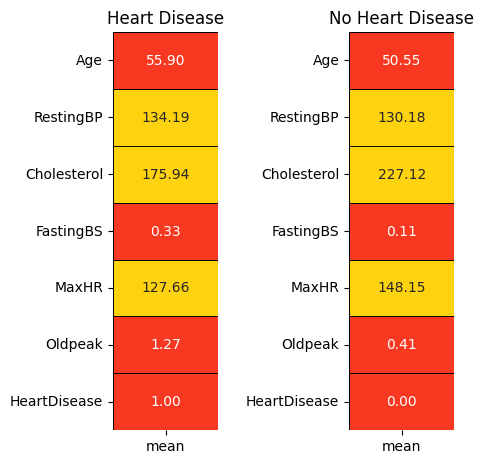
\includegraphics[width=\linewidth]{Figures/Outputs/mean-vals.png}
    \label{Mean value of all the features}
    \caption{Mean value of all the features present.}
\end{figure}